\chapter{Tetris}
\label{chap:cuatro}

La segunda mitad del siglo XX trajo consigo un avance tecnológico 
significativo como fue la integración gradual de las computadoras, como 
herramienta práctica para resolver problemas de forma rápida y eficiente. Los videojuegos 
fueron una consecuencia de un uso lúdico de estos aparatos electrónicos y sus 
reglas, fuente de curiosidad de investigadores y científicos. Desde su aparición, 
Tetris fue adoptado rápidamente como un videojuego icónico tanto en el ámbito de 
investigación científica como lúdico. 

\section{Historia}

A principio de la década de los ochenta, Alex Pajitnov trabajaba en un
laboratorio de cómputo para la Academia de Ciencias de la entonces Unión Soviética
como investigador en el área de inteligencia artificial. En junio de 1984
Pajitnov, impulsado por su gusto a los rompecabezas\footnote{En particular por
  el juego de figuras llamadas pentominó.} programó un conjunto de instrucciones
que dieron como bases las reglas del juego que llamó Tetris.

Por políticas de su gobierno y temiendo represalias debido a que programar
juegos no era parte de su trabajo, Pajitnov decidió no publicar su juego, sin
embargo, el código de Tetris se filtró hacia Hungría y poco a poco
abrió su paso hasta Estados Unidos, donde fue publicado, 
comercializado y vendido a millones de jugadores de videojuegos.

Para 1989 al menos seis compañías reclamaban los derechos del juego Tetris
para consolas de videojuegos, computadoras personales y equipos portátiles.
Con la eventual caída del bloque Soviético los derechos legales sobre Tetris,
lentamente regresaron a Pajitnov para comercializar su creación~\cite{tetris-history}.

\begin{figure}[h]
    \centering
    \setlength{\fboxrule}{1pt}
    \framebox{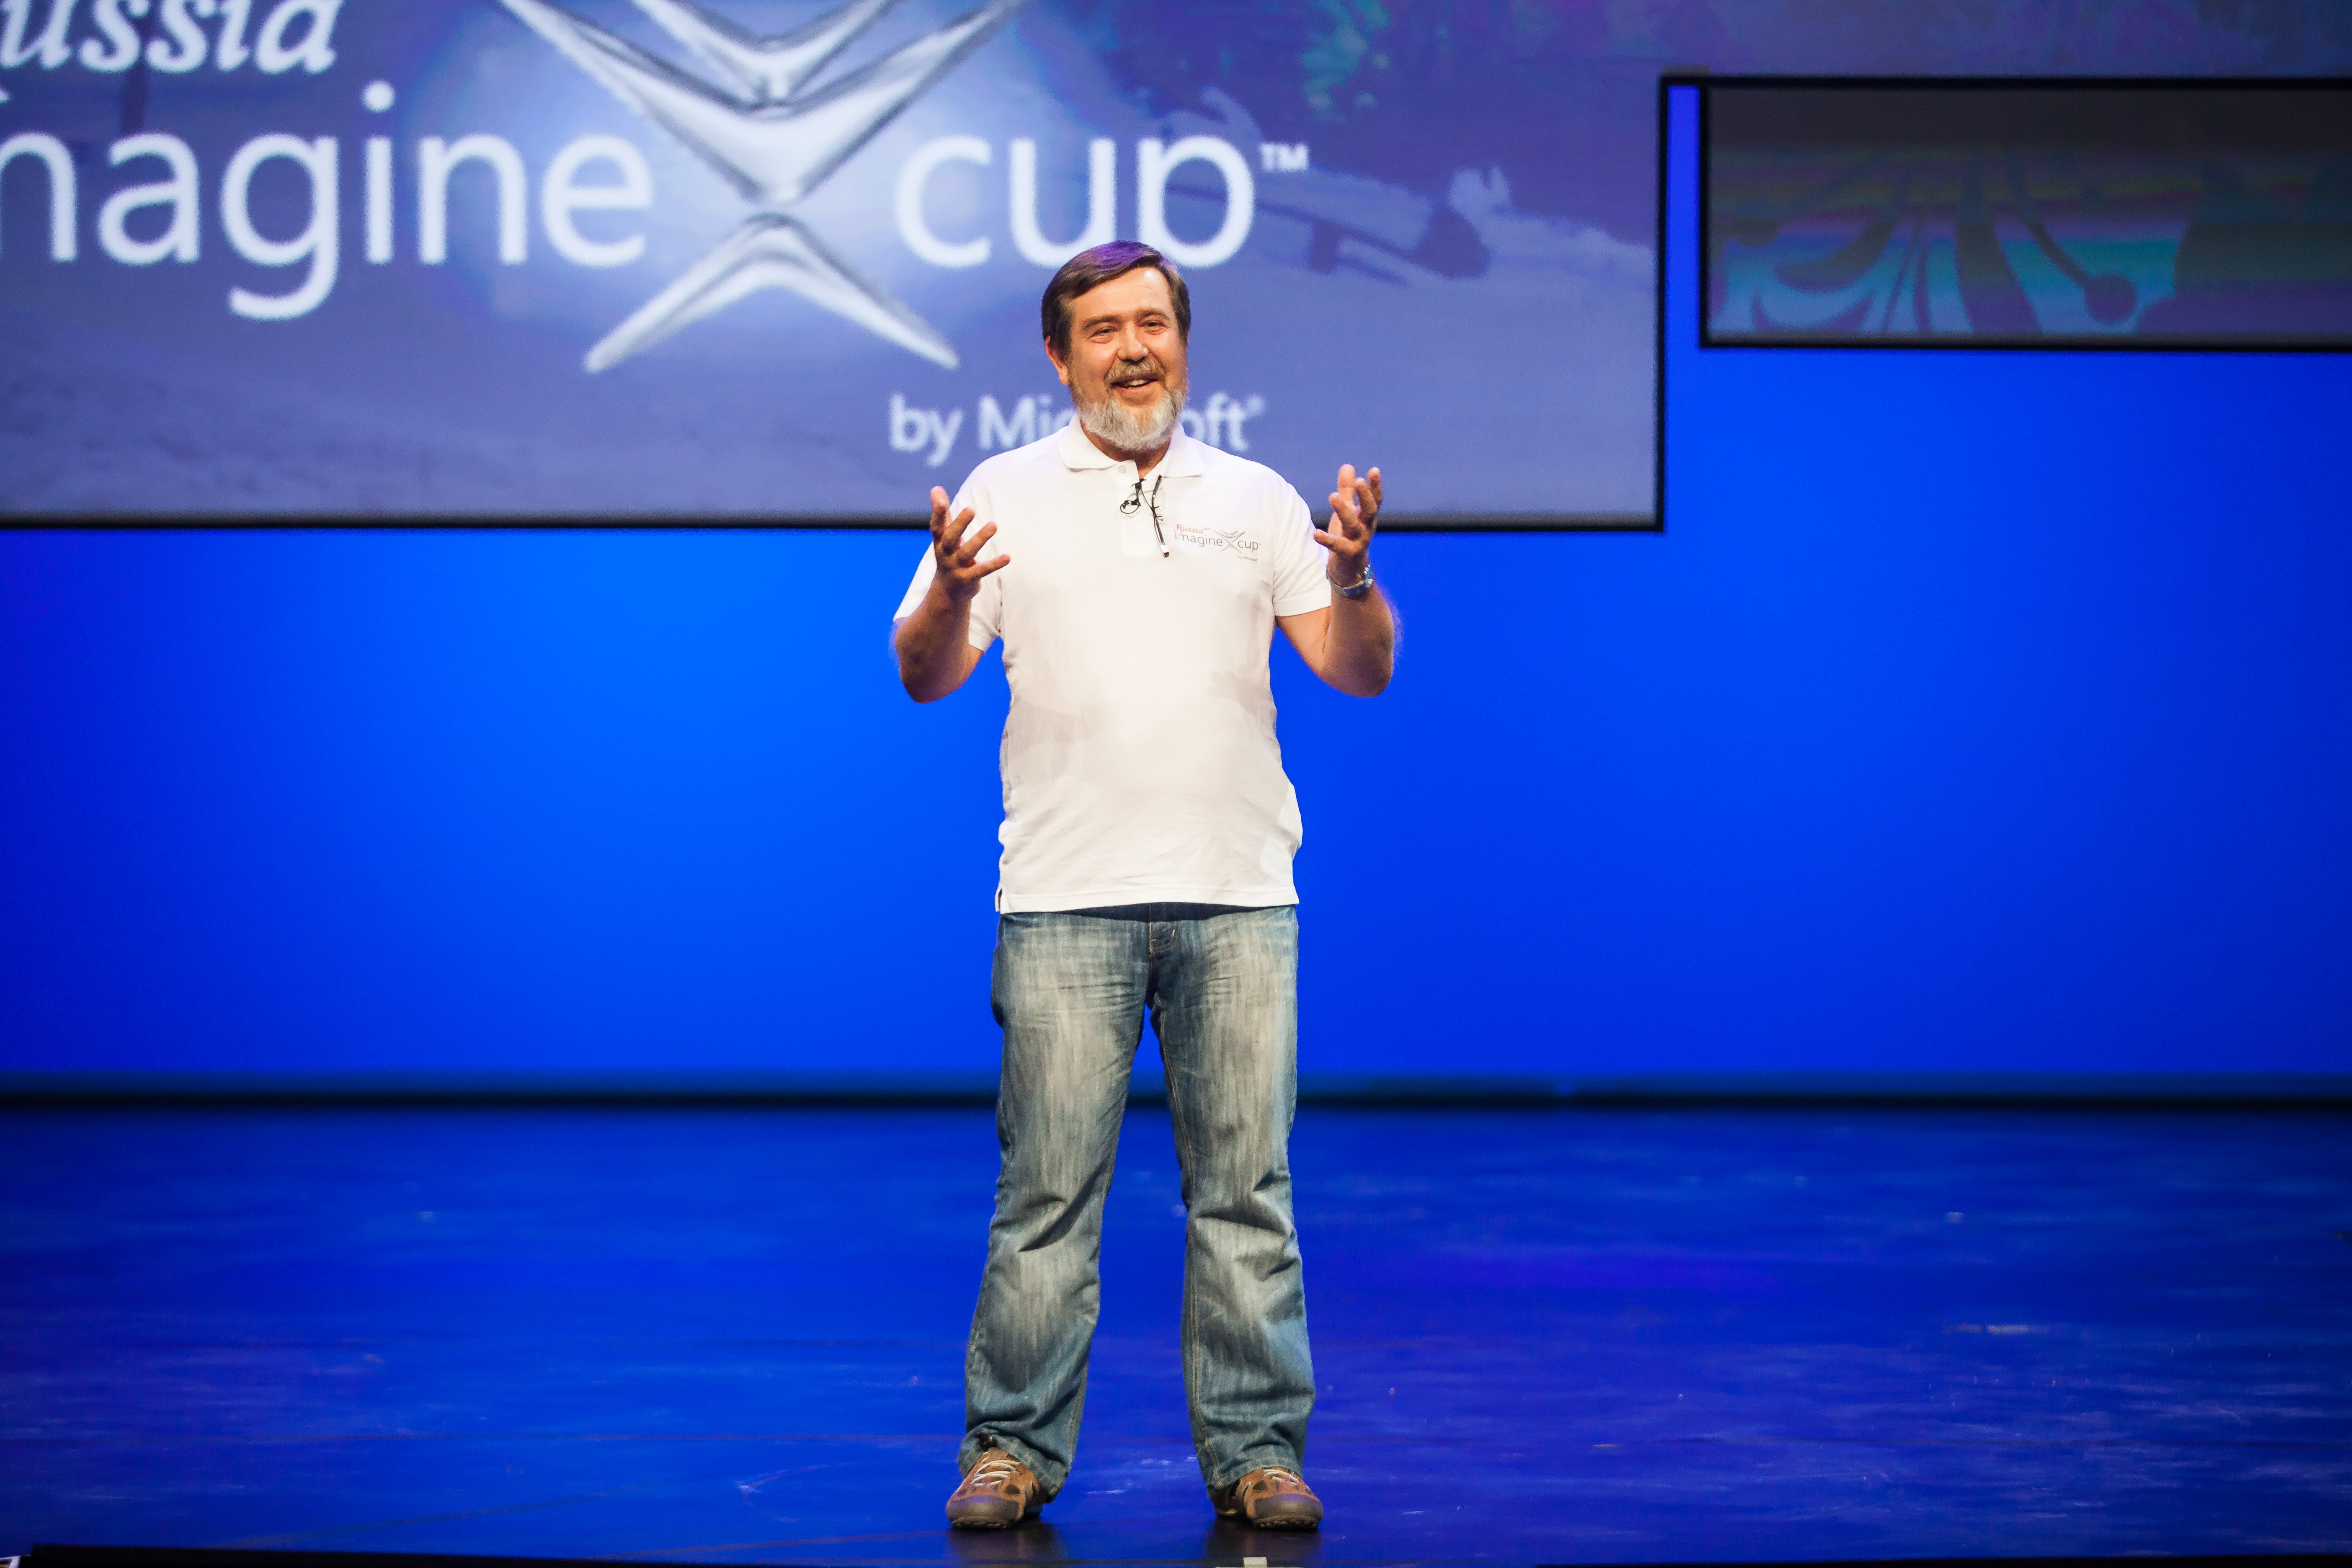
\includegraphics[width=\textwidth,height=5cm,keepaspectratio=true]{./images/Alexey_Pajitnov.jpg}}
    \caption{Alex Pajitnov, diseñador y creador de
    Tetris, en la final de la copa mundial 2013 de \textit{Image Microsoft}, en San Petesburgo, Rusia~\cite{WikipediaEN:AlexeyPajitnov}.}
    \label{fig:AlexPajitnov}
\end{figure}

Actualmente Tetris es uno de los videojuegos más vendidos de la historia con una
estimación de alrededor de 170 millones\footnote{Copias físicas y digitales.} de
copias vendidas y muchas variantes alrededor del mundo~\cite{tetris-numbers},
siendo la consola Game Boy, de la compañía Nintendo, su primer distribuidor
mayoritario~\cite{tetris-25-aniv}.

Desde el punto de vista matemático y computacional, Tetris ha planteado muchas
preguntas y planteamientos, como la posibilidad de jugar de manera infinita sin
perder\footnote{La pregunta \textit{¿sería posible jugar Tetris por siempre?}
fue enunciada en~\cite{Burgiel97howto} y la imposibilidad bosquejada.}
o las combinaciones de movimientos que posee un jugador. Tetris
ha sido objeto de estudio por diferentes campos como matemáticas, teoría de la
computación, teoría de algoritmos, psicología~\cite{Brzustowski_1992},
\cite{Burgiel97howto}, entre otros.

\section{Definición del problema}

Limitado por los gráficos de una computadora soviética llamada Electronika 60,
Pajitnov tomó la decisión de bajar la complejidad del juego de pentominó de~18
piezas, a uno de tetraminó de~7. Adicionalmente agregó lógica al juego como la
posibilidad de desaparecer líneas de piezas al ser completadas horizontalmente,
creando un juego simple y fácil de entender~\cite{tetris-history}, modificando
así el juego original.

\begin{figure}[h]
  \centering
      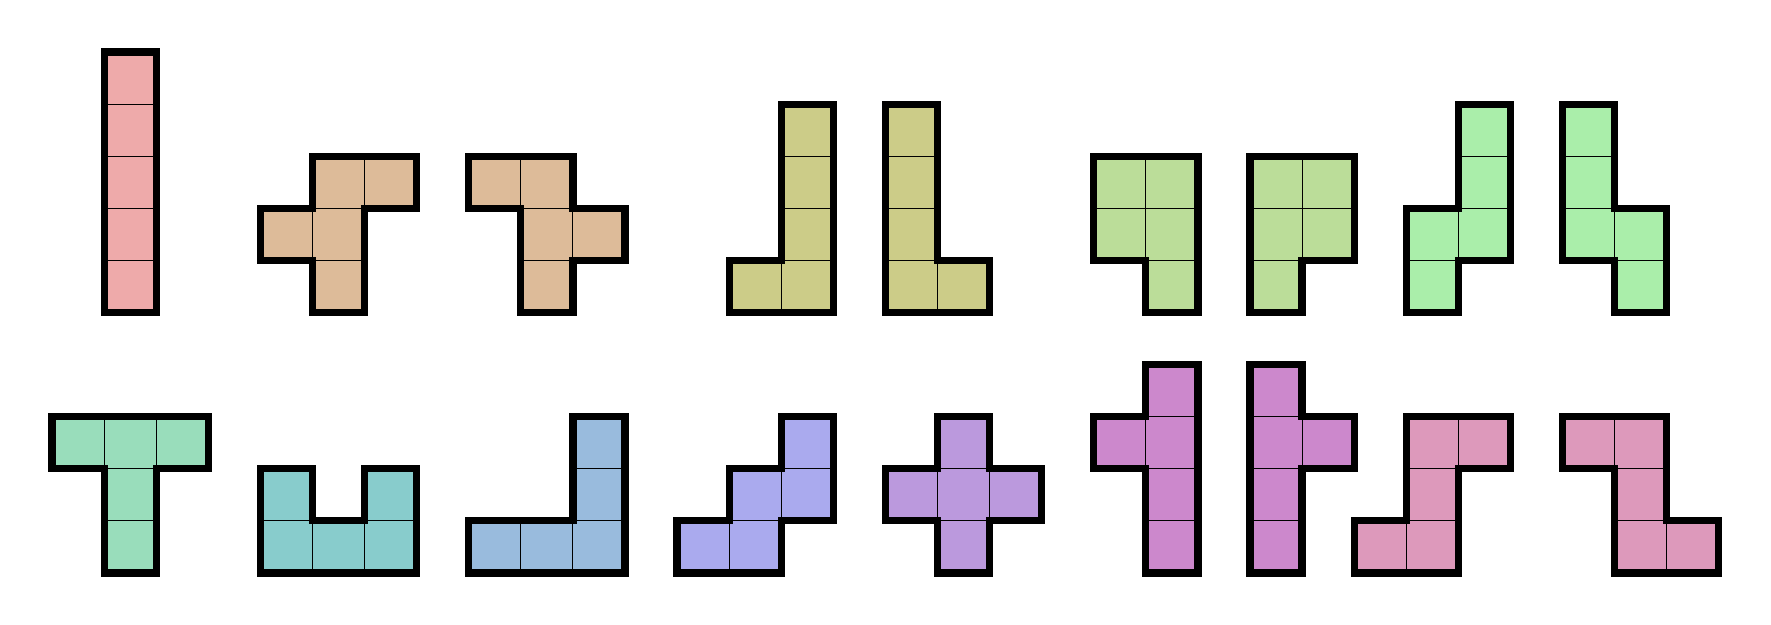
\includegraphics[width=0.8\textwidth]{./images/pentominoes}
    \caption{18 piezas del pentominó, juego original en el que se basó Alex
    Pajitnov que consiste en tratar de acomodar las 18 piezas en un
    tablero, sin dejar espacios~\cite{WikipediaEN:pentomino}.}
    \label{fig:Pentomino}
\end{figure}

La versión original del juego programada por Pajitnov hace uso de un tablero de
$10$ unidades de ancho por $20$ unidades de alto. En muchas versiones de Tetris
posteriores el tablero puede llegar a tener $n \times m$
unidades. Cuando el juego empieza, el tablero se encuentra vacío; inmediatamente
después la primera de las \textit{piezas}, que se les denomina tetraminós,
empiezan a aparecer en la parte superior del tablero.

Los tetraminós son un grupos de piezas geométricas conformada por cuatro
unidades cuadradas que se definen como \textit{celdas}. Cada celda ocupa
exactamente una unidad vacía del tablero y no pueden existir dos celdas en mismo
punto $(i \times j)$\footnote{A este punto también se puede ver como el espacio
  $(i,j)$ o la columna $j$, con la fila $i$.}. Después de aparecer en la
pantalla, las piezas bajan fila por fila, de manera pausada hasta llegar al
fondo del tablero o a un punto en el que ya no pueda bajar más debido a que se
sobrepondría a alguna otra pieza. Al ya no poder bajar más, el tetraminó
actual se mantiene en esa posición mientras un nuevo tetraminó, seleccionado
aleatoriamente dentro del grupo de siete posibles figuras (ver
\cref{fig:Tetrominos}) aparece en la parte medio superior del tablero para
ser de nuevo colocada en el tablero en alguna posición inferior.

\begin{figure}[h]
    \centering
    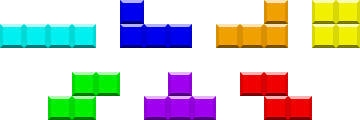
\includegraphics[width=0.6\textwidth]{./images/tetrominos}
    \caption{Los siete posibles tetrominós~\cite{WikipediaEN:tetrominos}.}
    \label{fig:Tetrominos}
\end{figure}


Los jugadores tienen a su disponibilidad la acción de rotar los tetraminós para
orientar las piezas mientras éstas caen. Otra acción que puede realizar el
jugador es mover las piezas a la columna derecha o izquierda y forzar a la 
pieza caer un nivel. Los jugadores
poseen un tiempo limitado para realizar estas acciones antes de que la pieza
sea empujada por la \textit{gravedad} simulada del juego a una fila inferior.

La mayoría de las implementaciones tienen típicamente un recuadro donde aparece
la siguiente pieza a jugar; cuando la pieza $i$ está siendo colocada en el
tablero, la pieza $(i + 1)$ es revelada en el cuadro. A ese cuadro se le llama 
\textit{cuadro de pista}~\cite{DBLP:journals/corr/cs-CC-0210020}.

Cuando toda una fila se encuentra llena de celdas de los tetrominós,
las celdas de los tetrominós en dicha fila son removidas del tablero y
las celdas de las piezas en filas superiores son desplazadas hacia niveles 
inferiores para llenar el espacio dejado por la fila removida. 
Un \textit{tetris} ocurre cuando cuatro filas son removidas al 
mismo tiempo. Si los jugadores no remueven
celdas lo suficientemente rápido, el tablero del juego se
quedará sin espacio para seguir colocando piezas y la partida
terminará~\cite{Burgiel97howto}.

Debido a los resultados obtenidos por~\cite{Burgiel97howto}, se sabe que es
imposible ganar el juego de Tetris, por lo que el objetivo principal del
jugador es maximizar la cantidad de puntos que se van acumulando durante la
partida. Estos puntos varían dependiendo de las acciones del jugador y la
interacción de las fichas en el tablero (como la desaparición de fichas o
realizar un \textit{tetris}).


\section{Un problema \textsl{NP}-completo}

En el año 2008, un equipo de computólogos publicó un artículo donde demuestran
que programar una computadora para que juegue a Tetris, es un problema \textsl{NP}-completo.
El objetivo de esta sección será enunciar, explicar los pasos y procedimientos
que la publicación~\cite{DBLP:journals/corr/cs-CC-0210020} usó, para demostrar
la \textsl{NP}-completez del juego de Tetris. El resultado de esta sección
justifica la implementación de la heurística al problema que aborda este
trabajo.

Para comenzar con la demostración, el equipo conformado por Erik D. Demaine,
Susan Hohenberger y David Liben-Nowell definieron una versión un poco diferente
al videojuego. El cambio más importante de la versión que se presenta en el artículo
es la clasificación de dos posibles flujos de información que pueden existir:
la versión que llaman \textit{offline} es aquella en la cual la entrada del programa
contiene la lista de las piezas de forma determinista, finita y ordenada que existirán
hasta un tiempo $T$. La versión \textit{online} es aquella en la que la
información de las piezas a jugar en un tiempo $T$ es sólo la pieza $P_{T}$
y, a lo más, el tetrominó $P_{T+1}$ dentro del cuadro de pista.

Aunque la demostración del problema es sobre la versión del juego
\textit{offline}, se supone en el artículo que la versión del juego \textit{online} es al menos
(hablando de complejidad computacional) tan difícil como la versión
\textit{offline}~\cite{DBLP:journals/corr/cs-CC-0210020,boumaza:hal-00926213}.
Mencionan los autores que es intuitivamente más fácil hacer jugar a la computadora con el conocimiento
total de los movimientos posteriores que debe realizar, así que la conclusión
de la \textsl{NP}-completez de la versión \textit{offline} indica la complejidad
de hacer jugar la versión \textit{online}.

Existen cuatro objetivos del juego que son demostrados, tratar de optimizarlos
es un problema \textsl{NP}-completo:

\begin{itemize}

\item Maximizar el número de filas removidas mientras se juega alguna secuencia.

\item Maximizar el número de piezas antes de que el juego se termine.

\item Maximizar el número de veces que se hace un \textit{tetris}.

\item Minimizar la altura de la columna más alta.
\end{itemize}

Para demostrar que los objetivos (y el juego) es \textsl{NP}-completo, primero
demuestran que el problema formal del juego, \texttt{TETRIS} es elemento de 
la clase \textsl{NP}; luego que la maximización
 del número de filas removidas es un problema
\textsl{NP}-duro; los demás puntos los demuestran reduciéndolos entre ellos.
La prueba inicial de la pertenencia a \textsl{NP}-duro que hacen los
autores incluye una reducción a partir del problema visto en el
\cref{sec:3-particion}.

\subsection{Formalización del juego}
\label{subsec:formalizacion}

Las reglas de Tetris son definidas rigurosamente con el fin de transparentar
la reducción y demostraciones hechas con las operaciones y propiedades del
juego. El modelo formal propuesto consiste en los siguientes
agentes y será respetado en su mayoría durante la implementación de este trabajo:

\begin{itemize}[leftmargin=0.8cm,align=left]
\item[\textbf{Tablero. }] El tablero es una matriz de $n$ filas por $m$ columnas
enumeradas de abajo hacia arriba y de izquierda a derecha. La casilla
$\langle i, j \rangle$ del tablero puede estar en dos estados: \textit{ocupada} o
\textit{libre}. En un tablero válido no existen filas $c$ tal que
$\langle c,k \rangle$ con $k\in \{0,1,...,m\}$ tenga
\textit{ocupadas} a todas sus casillas. Tampoco existen filas completamente vacías que se
encuentren por debajo de alguna casilla ocupada.

\item[\textbf{Piezas. }] Los ya definidos tetraminós como los mostrados en
la \cref{fig:Tetrominos}. Cada tetraminó tendrá ahora la estructura de la
forma $P = \langle t, o, \langle i,j \rangle, f \rangle$ donde cada elemento es
respectivamente:

\begin{enumerate}
        \item Un tipo de pieza. De izquierda a derecha en la  
        \cref{fig:Tetrominos}, el tipo de pieza sería:
        \texttt{I}, \texttt{RS}, \texttt{LG}, \texttt{T},
        \texttt{RG}, \texttt{LS} y \texttt{Sq}.

        \item Una orientación dada en grados: $0^{\circ}, 90^{\circ}, 180^{\circ}$ o $270^{\circ}$.

        \item Una posición $\langle m_{c},k_{c} \rangle$ donde se encuentre la casilla
        centro de la pieza.

        \item Un valor de \texttt{FIJO} o \texttt{MOVIBLE}.
\end{enumerate}

Adicionalmente, cada tipo de pieza posee un centro. Se seleccionará una
casilla y esa casilla será considerada el centro de la pieza al ser rotada.

En el estado inicial, las piezas se encuentran en una orientación $0^{\circ}$,
la posición inicial es la $\langle m ,\lfloor n/2 \rfloor \rangle$ y la pieza tiene
el valor de \texttt{MOVIBLE}.

\item[\textbf{Rotación. }] Un modelo de rotación que es una función computable
$R: \langle P, \theta, B \rangle \mapsto P'$, donde $P$ y $P'$ son orientaciones
de las piezas, $\theta \in \{-90^{\circ}, 90^{\circ}\}$ es el ángulo de
rotación y $B$ es el tablero. El artículo define las siguientes
condiciones para $R$:

\begin{enumerate}
\item Si $P = \langle t, o, \langle i,j \rangle, f\rangle$ y la rotación es válida,
entonces $P' = \langle t, (o + \theta) \mod 360^{\circ}, \langle i,j \rangle, f\rangle$
para algún $\langle i,j \rangle$. Si la rotación no es válida, entonces $P' = P$.

\item Para determinar la validez de una rotación, $R$ sólo necesita examinar
una vecindad de tamaño $O(1)$ de la pieza $P$.

\item Si todos las casillas de la vecindad de $P$ están vacías, se dice que la
rotación es válida o legal.

\item Si la rotación es legal, $P'$ no debe ocupar ninguna casilla ya ocupada
por algún otro tetrominó en $B$.

\end{enumerate}

\item[\textbf{Reglas del juego. }] La única regla para las fichas con estado
\texttt{FIJO} es que no existen movimientos válidos para ésta. Las piezas de
la forma $P = \langle t, o, \langle i,j \rangle, \texttt{MOVIBLE}\rangle$ en un
tablero $B$, tienen el siguiente conjunto de \textit{movimientos}
\footnote{Llámese ``movimiento'' a un elemento del conjunto de acciones posibles 
del jugador, en un límite de tiempo.} disponibles:

\begin{enumerate}
\item Rotación en dirección a las manecillas del reloj. $R(P, 90^{\circ}, B)$.

\item Rotación contraria a las manecillas del reloj. $R(P, -90^{\circ}, B)$.

\item Desplazamiento a la izquierda.
$P' = \langle t, o, \langle i - 1,j \rangle, \texttt{MOVIBLE}\rangle$.

\item Desplazamiento a la derecha.
$P' = \langle t, o, \langle i + 1,j \rangle, \texttt{MOVIBLE}\rangle$.

\item Deja caer. $P' = \langle t, o, \langle i,j - 1 \rangle, \texttt{MOVIBLE}\rangle$.

\item Asignar estado. Si existe al menos una casilla ocupada debajo de $P$,
entonces $P' = \langle t, o, \langle i,j \rangle, \texttt{FIJO}\rangle$.
\end{enumerate}

Para las reglas del tablero, se define una trayectoria $\sigma$ de una pieza $P$.
La trayectoria es una secuencia de movimientos válidos del estado inicial de la
pieza, hasta la asignación del estado \texttt{FIJO} de $P$. El resultado de una
trayectoria sobre el tablero $B$, es un tablero nuevo $B'$ definido con las
siguientes características:

\begin{enumerate}
\item El tablero nuevo $B'$ es inicialmente $B$ con la figura $P$.

\item Si $P$ tiene el estado de \texttt{FIJO} y para alguna fila $r$, cada
casilla de $r$ está ocupada en $B'$, las celdas
de los tetrominós en $r$ son removidos. Para cada $r' \geq r$, se reemplaza a
la fila $r'$ en $B'$ con la fila $r' + 1$ de $B'$. Múltiples filas pueden ser
removidas con una sola trayectoria.

\item Si existe alguna casilla ocupada en $B'$ donde debería estar la siguiente
pieza en su estado inicial, el jugador pierde.

\end{enumerate}

Para un juego $\langle B_{0}, P_{1}, ..., P_{p} \rangle$, una secuencia de
trayectorias $\Sigma$ es una secuencia $B_{0},\sigma_{1},B_{1},...,\sigma_{p},B_{p}$
tal que para cada $i$, la trayectoria de la pieza $P_{i}$ aplicado al tablero
$B_{i-1}$, genera el tablero $B_{i}$.

\item[\textbf{Problema formal}] Aunque el artículo contempla varios objetivos
previamente mencionados a optimizar, el problema de decisión con el objetivo
$\Phi$ del juego de Tetris, $\texttt{TETRIS}[\Phi]$, es enunciado
formalmente como sigue:

\begin{itemize}

\item \textbf{Input:} Un juego de Tetris de la forma 
$\mathcal{G} = \langle B, P_{1}, P_{2}, ..., P_{p} \rangle$.

\item \textbf{Output:} ¿Existe la secuencia de trayectorias $\Sigma$ tal que 
$\Phi(\mathcal{G}, \Sigma)$ no resulte en una partida perdida?

\end{itemize}

\end{itemize}

Una vez definido minuciosamente el modelo formal de Tetris, incluyendo las
reglas y los objetos que participan en una partida, se procede a discutir su
complejidad.

\subsection{La clasificación de \texttt{TETRIS}}

Se sabe por las definiciones del \cref{sec:np-def}, que para que
\texttt{TETRIS} esté en \textsl{NP}-completo, debe cumplir con que
\texttt{TETRIS} $\in$ \textsl{NP}-duro y $\texttt{TETRIS} \in \textsl{NP}$.

Para llegar a la conclusión de la \textsl{NP}-completez, los autores tuvieron
que proponer y demostrar ciertos lemas y teoremas enunciados a continuación:

\begin{itemize}[leftmargin=0.5cm,align=left]

\item[\textbf{Teorema 2.1}] Para cada objetivo \textit{acíclico}\footnote{Se dice que una
función objetivo $\Phi$ es acíclica si para todo juego $\mathcal{G}$ en los que 
exista una trayectoria $\Sigma$ tal que $\Phi(\mathcal{G},\Sigma)$ no
pierde, entonces existe una trayectoria $\Sigma'$ tal que
$\Phi(\mathcal{G},\Sigma')$ no pierde y no existen estados repetidos de
las piezas en $\Sigma'$.} comprobable $\Phi$, se tiene
que \texttt{TETRIS}[$\Phi$] $\in$ \textsl{NP}.

En el artículo se da un algoritmo \textsl{NP} para \texttt{TETRIS}[$\Phi$]. Los autores
argumentan que dado una $\Sigma$ aleatoria, se puede verificar que
$\Phi(\mathcal{G}, \Sigma)$, en tiempo polinomial\footnote{Se nombrará de
manera genérica a la función de verificación en tiempo polinomial, función
\texttt{POLY}.}  ya que también se puede verificar
$\texttt{POLY}(|\mathcal{G}|, |\Sigma|) = \texttt{POLY}(|\mathcal{G}|)$
debido a que cada de las $p$ trayectorias en $\Sigma$ contiene a lo más
$4 \cdot |B| + 1$ estados a verificar, $|B| = n\times m$ con $n$ y $m$ el número de filas
y columnas de cada tablero.

\item[\textbf{Lema 2.2}] El objetivo \textit{k-filas-removidas}\footnote{
$\texttt{k-filas-removidas}:\mathcal{G} \times \Sigma \rightarrow \mathds{N}$
nos regresa el número de filas removidas durante un juego de Tetris.} es
\texttt{POLY} verificable y acíclico.

La corta demostración de este lema se realiza mediante la argumentación
de que \texttt{k-filas-removidas} es acíclico porque sólo depende del estado
de cada pieza que es colocada al final de cada trayectoria en el tablero.
Es \texttt{POLY} verificable ya que sólo es necesario recorrer cada tablero que
regrese cada trayectoria en a lo más $O(m \cdot n \cdot |\Sigma|)$.

\item[\textbf{Teorema 3.1}] \texttt{3-PARTITION} es un problema \textsl{NP}-completo.

Este teorema es discutido en la \cref{sec:3-particion} y demostrado
en~\cite{Garey:1990:CIG:574848}.

\item[\textbf{Teorema 3.2}] El juego $\mathcal{G}(\mathcal{P})$ es polinomial
respecto a $\mathcal{P}$.

Para explicar este teorema, primero hay que explicar la decisión que tomaron
Demaine,  Hohenberger y Liben-Nowell en su artículo para el problema de reducción:

Los autores decidieron crear la reducción del problema \texttt{3-PARTITION}
debido a su propiedad de ser fuertemente \textsl{NP}-completo; esto incluye
valores de entrada $a_{i}$ y $T$ unitarios. También de enfocan en instancias
específicas de \texttt{3-PARTITION}:

\begin{enumerate}
\item Para cada conjunto $S \subseteq \{a_{1},...,a_{3s}\}$, si $\sum_{a_{i} \in S} a_{i} = T$
entonces $|S| = 3$.

\item $T$ es par.

\item Si $\sum_{a_{i} \in A_{j}} a_{i} \neq T$ entonces
$\left|T - \sum_{a_{i} \in A_{j}} a_{i} \right| \geq 3s$.
\end{enumerate}

Dada una instancia $\mathcal{P} = \langle a_{1}, ..., a_{3s},T \rangle$ que
cumpla las tres condiciones de arriba, $\mathcal{G}(\mathcal{P})$ es un juego
de Tetris que elimina a todas las piezas si $\mathcal{P}$
tiene como respuesta un valor booleano de \texttt{TRUE}.

El tamaño del tablero y el número de piezas dependerá de los valores $S$ y
$T$ del problema de la \texttt{3-PARTITION}: el tamaño del tablero resultante
de $\mathcal{G}(\mathcal{P})$ es de $6T + 22 + 3s +  O(1)$ filas por $6s + 3$
columnas, mientras que el número de piezas totales del juego será de:

\begin{displaymath}
\sum\limits_{i=1}^{3s}[3 + 5a_{i} +2] + s + 1 + \left( \frac{3T}{2} + 5 \right)
= 16s + 5sT + \frac{3T}{2} + 6.
\end{displaymath}

Los valores $a_{i}$ y $T$ están representados como valores unarios (por la
naturaleza del sistema de conteo de casillas en el tablero) por lo que
se puede suponer siempre una transformación polinomial a la hora de construir
el juego conforme a la opinión de los autores de la demostración.

\item[\textbf{Teorema 4.1} (Completez)]  Para cada instancia
$\mathcal{P}$ que tenga como respuesta un valor booleano de \texttt{TRUE} del
problema de la \texttt{3-PARTITION}, existe una secuencia de trayectorias
$\Sigma$ que \textit{limpie}\footnote{En este contexto, limpiar el tablero
tiene el significado de mantener el juego sin piezas, es decir, que todas
las piezas jugadas sean en algún punto removidas del tablero.}
el tablero $\mathcal{G}(\mathcal{P})$ sin que el juego termine, o el jugador
pierda. \\% \linebreak

 \begin{figure}[h!]
\centering
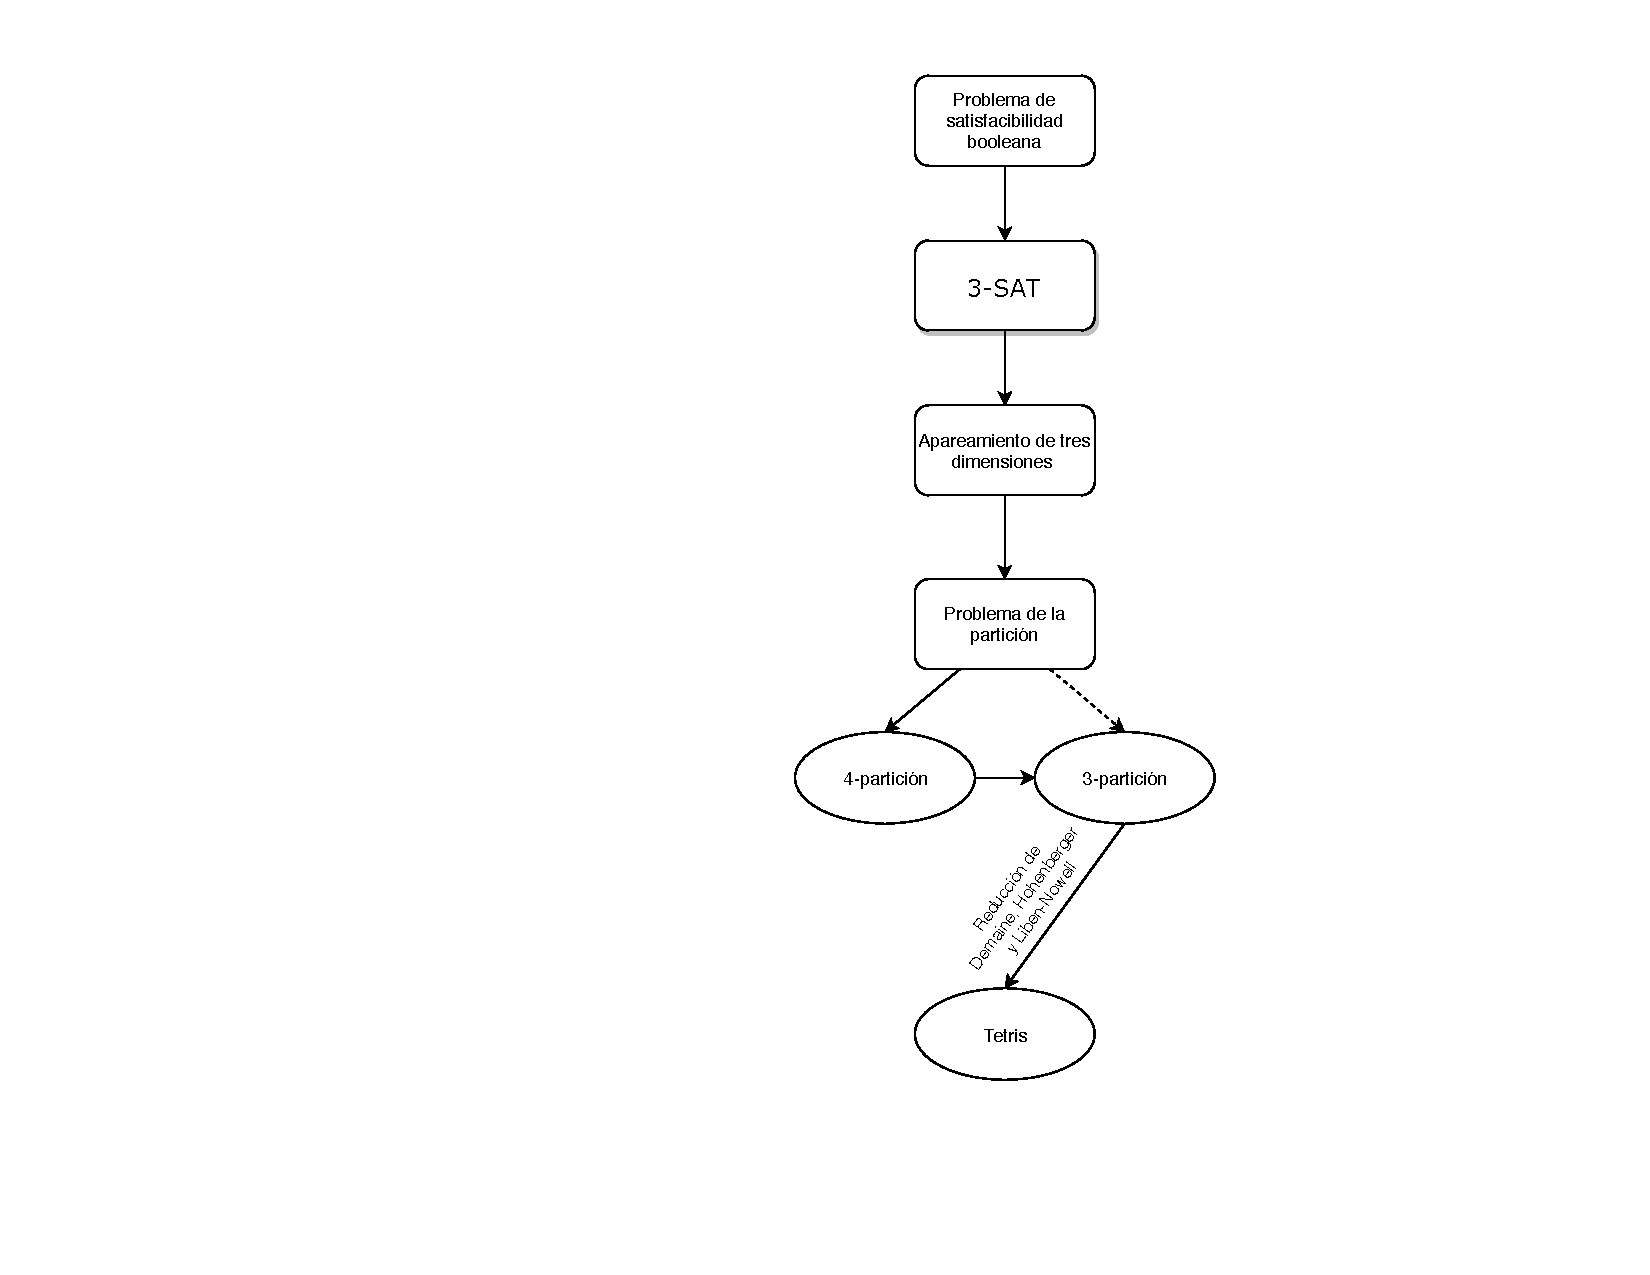
\includegraphics[width=0.4\textwidth,keepaspectratio,trim={12cm 6cm 7cm 1cm}]{./images/4_3_1.pdf}
\linebreak\linebreak\linebreak\linebreak\linebreak\linebreak
\caption{Extensión del diagrama de la \cref{fig:secuenciaNP} de las reducciones
polinomiales desde \texttt{SAT} hasta Tetris con $\mathcal{G}(\mathcal{P})$.}
\end{figure}

La forma que proceden en esta demostración es partiendo por la condición de
veracidad de \texttt{3-PARTITION}; aprovechan la partición
de los conjuntos $A_{i}$ para asociar a los tetrominós con algún número,
 acomodarlos en algo que los autores llaman \textit{cubetas}, que son
 divisiones del tablero que se le asigna a cada $A_{i}$ y así, asegurar no dejar
 espacios casillas sin llenar. De manera bastante ilustrativa construyen estas
 secuencia de piezas o configuraciones donde se aseguran no existan huecos en las filas,
 produciendo así su \textit{limpieza} y remoción del tablero.

Dada la reducción propuesta
$\texttt{3-PARTITION} \leq_{\mathcal{G}(\mathcal{P})} \texttt{TETRIS}$,
 la demostración dentro del artículo y las definiciones de
 \cite{arora2009computational} en la \cref{sec:np-def}, se puede afirmar que
 \texttt{TETRIS} $ \in $ \textsl{NP}-duro.

\item[\textbf{Lema 5.10}] El modelo de rotación propuesto es suficiente.

Cubriendo todos los posibles casos con los siete tetraminós, los autores
muestran que no existe combinación de rotaciones en el que las piezas
puedan (o piezas diferentes a ellas no puedan) llenar ciertos espacios del
tablero.

\item[\textbf{Teorema 5.16}] Si existe una estrategia válida para
$\mathcal{G}(\mathcal{P})$, entonces $\mathcal{P}$ es una instancia de
\texttt{3-PARTITION} que tiene respuesta un valor booleano de \texttt{TRUE}.

El artículo, va un poco más allá y plantea, discute y demuestra la propiedad
de que la robustez o exactitud\footnote{Viene del inglés \textit{soundness}.},
que significa que cualquier solución encontrada sea correcta.

Inmediatamente después de esta última demostración, el artículo enuncia como
consecuencia a todos los teoremas y lemas enunciados arriba, el siguiente
teorema:

\item[\textbf{Teorema 5.17}] \texttt{TETRIS}[\textit{k-filas-removidas}] es \textsl{NP}-completo.

Habría que recordar la definición que se enunció en el \cref{sec:np-def}; dice
que para que un problema esté dentro de la clase \textsl{NP}-completo, debe cumplir
que esté tanto en \textsl{NP} y en \textsl{NP}-duro. Estas propiedades se demuestran
en el \textbf{Teorema 3.1}. La parte de pertenencia a \textsl{NP}-duro se construye
por el \textbf{Teorema 4.1}, usando la reducción, los teoremas 2.1, 3.1, 3.2 y
5.16 y los lemas 2.2 y 2.10 se concluye que
\texttt{TETRIS}[\textit{k-filas-removidas}] $\in$ \textsl{NP}-completo.

\end{itemize}

Si bien, el artículo no termina con este teorema y va más allá, demostrando la
complejidad de cada uno de los objetivos a optimizar, para propósitos de este
trabajo, es suficiente este resultado por lo que en los capítulos posteriores
se habla de herramientas técnicas y la implementación del problema.

%%% Local Variables:
%%% mode: latex
%%% TeX-master: "../main"
%%% End:
